\documentclass[12pt,AutoFakeBold]{article} 

\usepackage[智能数据挖掘]{XDUreport}  % 科目名称
\problem{KDD CUP 网络入侵数据集小波分解}  % 请在此处填写问题内容
% 其他参数在宏包中进行更改,其中学院,班级,姓名,学号均在sty宏包内进行更改
% \usepackage{fourier}  % 这是 fourier 字体,更柔和 

%% 如果你需要中文的一级标题编号,如“一、”、“二、”等,请把下面两行取消注释
% \RequirePackage{zhnumber} % change section number to chinese
% \titleformat{\section}{\Large\bfseries\rmfamily}{\zhnum{section}、}{0em}{}

% 文档开始
        
\begin{document}

\maketitle
\setcounter{tocdepth}{2}

\tableofcontents  % 生成目录

% 正文标题
\makeatletter
\begin{center}
    \LARGE \textbf{\textsf{\@problem}}
\end{center}
\makeatother

% 正文开始

\section{KDD CUP99 数据集简介}

这是用于第三届国际知识发现和数据挖掘工具竞赛的数据集,该竞赛与 KDD-99 第五届知识发现和数据挖掘国际会议同时举行。竞赛任务是建立一个网络入侵检测器,一个能够区分“坏”连接(称为入侵或攻击)和“好”正常连接的预测模型。该数据库包含一组要审计的标准数据,其中包括在军事网络环境中模拟的各种入侵。由于数据集较大,我使用完整数据 10\% 的子集来进行实验。

\section{原理分析}

\subsection{小波变换}

在进行深度学习训练时会使用到大量的数据,这些数据中有会存在一些噪声,小波变换 (Wavelet Transform, WT) 可以用来去除数据中的噪声。小波变换继承和发展了短时傅立叶变换局部化的思想,同时又克服了窗口大小不随频率变化等缺点,能够提供一个随频率改变的“时间-频率”窗口,是进行信号时频分析和处理的理想工具。小波变换有两个变量:尺度 $a$ 和平移量 $b$。尺度 $a$ 控制小波函数的伸缩,平移量 $b$ 控制小波函数的平移。尺度就对应于频率 (反比),平移量 $b$ 就对应于时间。
%
\begin{equation}
w(a, b)=\frac{1}{\sqrt{a}} \int_{-\infty}^{+\infty} f(t) \cdot \psi\left(\frac{t-b}{a}\right) d t
\end{equation}

小波分解的意义就在于能够在不同尺度上对信号进行分解,而且对不同尺度的选择可以根据不同的目标来确定。

对于许多信号,低频成分相当重要,它常常蕴含着信号的特征,而高频成分则给出信号的细节或差别。人的话音如果去掉高频成分,听起来与以前可能不同,但仍能知道所说的内容;如果去掉足够的低频成分,则听到的是一些没有意义的声音。在小波分析中经常用到近似与细节。近似表示信号的高尺度,即低频信息;细节表示信号的低尺度,即高频信息。因此,原始信号通过两个相互滤波器产生两个信号。

通过不断的分解过程,将近似信号连续分解,就可以将信号分解成许多低分辨率成分。理论上分解可以无限制的进行下去,但事实上,分解可以进行到细节(高频)只包含单个样本为止。因此,在实际应用中,一般依据信号的特征或者合适的标准来选择适当的分解层数。

\subsection{离散小波变换}

在数字图像处理中,需要将连续的小波及其小波变换离散化。一般计算机实现中使用二进制离散处理,将经过这种离散化的小波及其相应的小波变换成为离散小波变换 (Discrete Wavelet Transform, DWT)。实际上,离散小波变换是对连续小波变换的尺度、位移按照 2 的幂次进行离散化得到的,所以也称之为二进制小波变换。

\section{实验过程}

首先导入数据集并预处理添加属性名,用 \lstinline[language=Python]|DataFrame._get_numeric_data Examples| 获取定量型数据。

然后使用 pywt 库中的单级离散小波变换函数 \lstinline[language=Python]|cA, cD = pywt.dwt(data, wavelet, mode='symmetric', axis=-1)|,其中 cA 表示近似系数(approximation coefficients),cD 表示细节系数(detail coefficient),一般近似系数代表信号中的低频信息,细节系数代表信号中的高频信息,低频信息则代表整段信号的整体特征,高频信息则代表信号中的细节特征,对于 axis 参数,axis = 0 代表对横轴操作,也就是第0轴;
axis = 1 代表对纵轴操作,也就是第1轴。实验中我采用 db1 小波基分解,具体结果见附录。 

\includepdfset{pagecommand={\thispagestyle{fancy}}} 
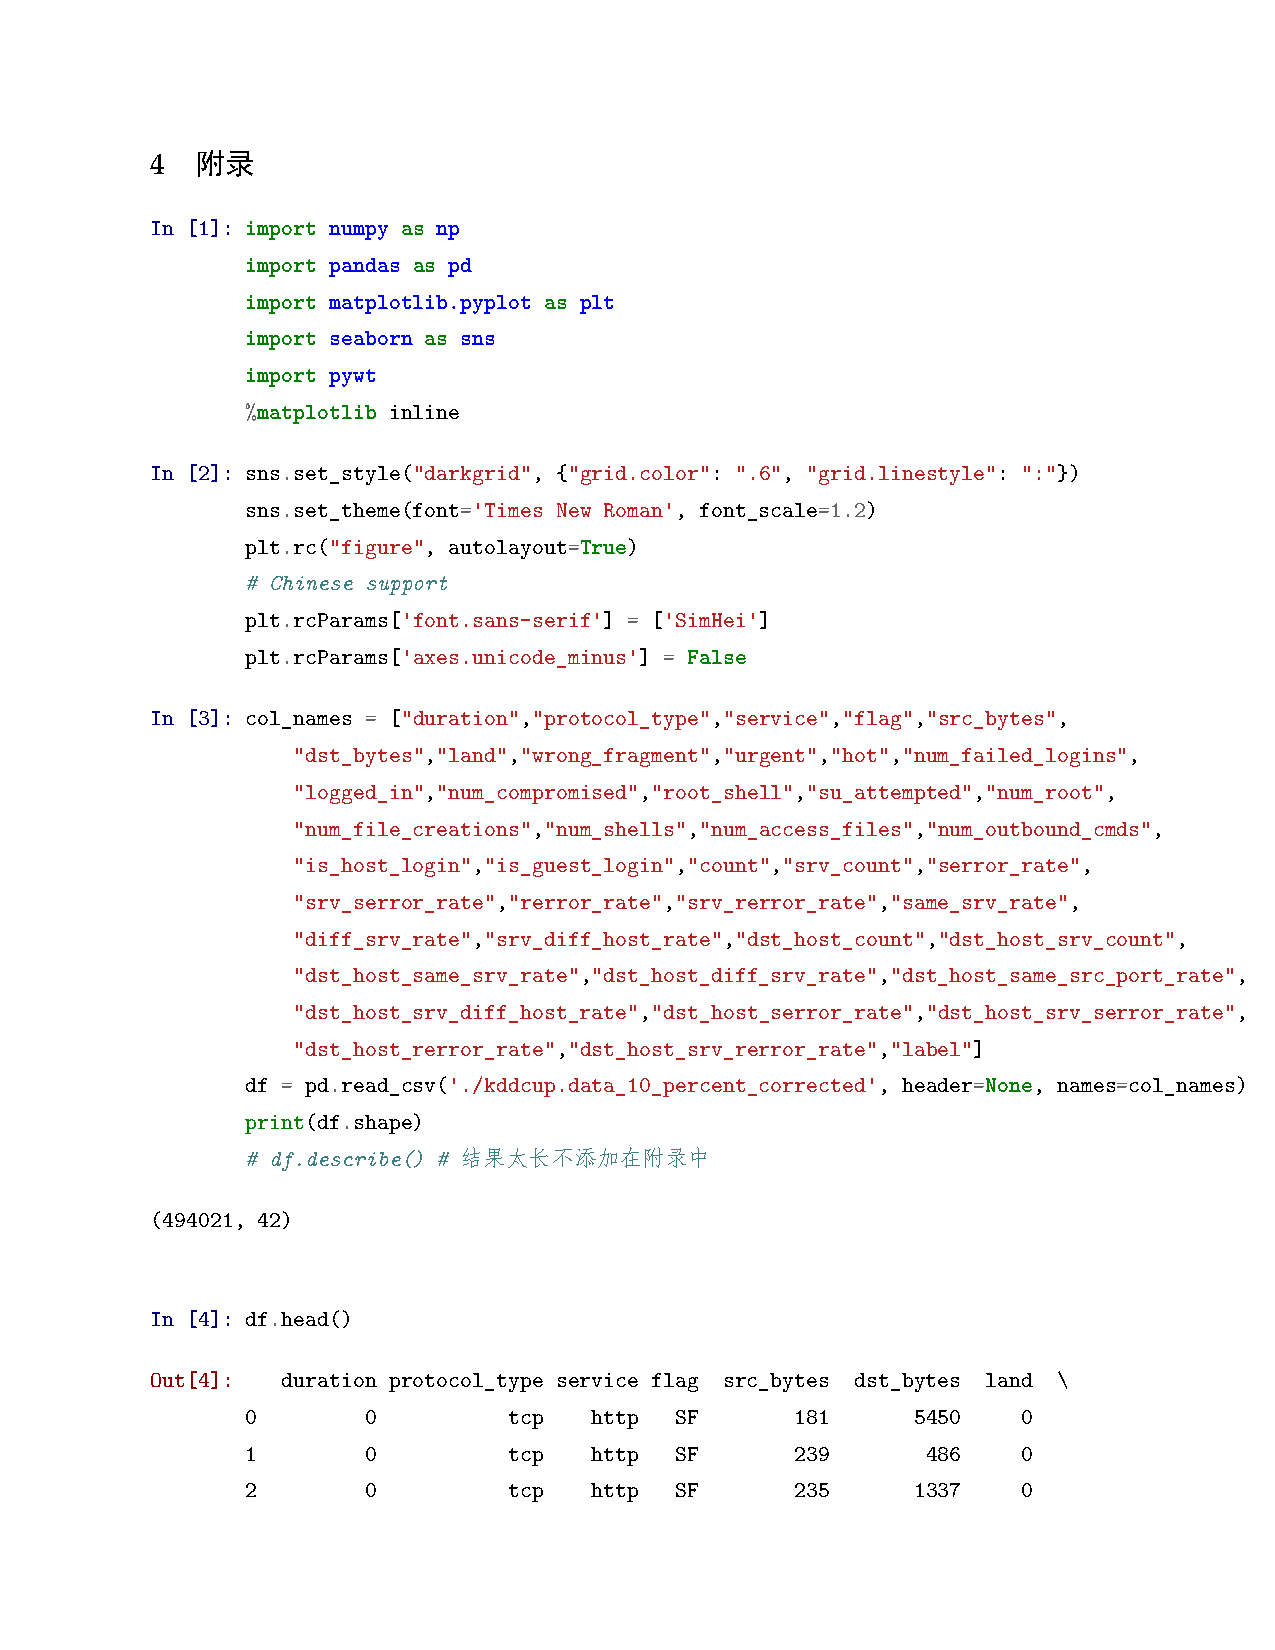
\includepdf[addtotoc={1,section,1,附录,appendix}, pages={1-4}]{Wavelet_Transform.pdf}

% % 参考文献,此处以 MLA 引用格式为例

% \begin{thebibliography}{9}
%     \bibitem{1} Clemente, Filipe Manuel, et al. "General network analysis of national soccer teams in FIFA World Cup 2014." \emph{International Journal of Performance Analysis in Sport} 15.1 (2015): 80-96.
%     \bibitem{3} Dijkstra, Edsger Wybe. "A Note on Two Problems in Connexion With Graphs." \emph{Numerische Mathematik} 1(1959):269-271.
%     \bibitem{4} Ahnert, Sebastian E., et al. "Ensemble approach to the analysis of weighted networks.." \emph{Physical Review E} 76.1 (2007).
%     \bibitem{5} Wong, J. A. Hartiganm. A. . "Algorithm AS 136: A K-Means Clustering Algorithm." \emph{Journal of the Royal Statistical Society. Series C (Applied Statistics)} 28.1(1979):100-108.
%     \bibitem{6} Buldu, J. M., et al. "Defining a historic football team: Using Network Science to analyze Guardiola’s F.C. Barcelona." \emph{Scientific Reports} 9.1 (2019): 1-14.
%     \bibitem{7} \emph{Balotelli sends Italy past Germany}. (2012). Retrieved December 10, 2014, from\url{https://www.uefa.com/uefaeuro/season=2012/matches/round=15174/match=2003379/index.html}
%     \bibitem{8} Sigari, Mohamad Hoseyn, et al. "Counterattack detection in broadcast soccer videos using camera motion estimation." \emph{international symposium on artificial intelligence} (2015): 101-106.
%     \bibitem{9} Abdelmahmoud Hassan Elsheikh. \emph{Effect of Leadership Intensity on Integrating Some Formal and Informal Organizational Efforts for Community Development in Khartoum Province}. 2016.
% \end{thebibliography}


% \includepdf[pages={1,2}]{Memo.pdf} 
% 可以直接导入pdf页面
% \newpage
% \begin{appendices}  % 附录环境
% \section{附录}
% \end{appendices}

\end{document}  % 结束